\documentclass{beamer}
\title{Constructing Lagrangian torus fibrations}
\author{Jonny Evans}
\date{joint with Mirko Mauri}
\include{beamer-head}
\begin{document}
\maketitle
\begin{frame}
\begin{overprint}
\onslide<1>
\begin{Theorem}[Gross 1999]\label{thm:gross}
Many Calabi-Yau 3-folds admit topological torus
fibrations over \(S^3\) with singular fibres over a
trivalent graph.
\end{Theorem}
\onslide<2>
\begin{block}{Question}
\begin{itemize}
\item Can we make these fibrations Lagrangian?
\item Even just (semi-)locally?
\end{itemize}
\end{block}
\onslide<3>
\begin{block}{Positive vertex: Yes!}
\begin{align*}
F&\colon\CC^3\setminus\{xyz-1=0\}\to\RR^3\\
F(x,y,z)&=\left(|x|^2-|y|^2,|x|^2-|z|^2,|xyz-1|\right)
\end{align*}
\end{block}
\onslide<4>
\begin{block}{Negative vertex: ?}
\[F\colon\CC^3\setminus\{(xy-z-1)z=0\}\to\RR^3?\]
\end{block}
\onslide<5>
\begin{block}{Negative vertex: Yes!}
\[F\colon\CC^3\setminus\{(xy-z-1)z=0\}\to\RR^3\]
\end{block}


\end{overprint}
\begin{overprint}
\onslide<1-4>
\begin{center}
\includegraphics[width=250pt]{discriminant}
\end{center}
\onslide<5>
\begin{center}
\includegraphics[width=200pt]{theorems}


\end{center}
\end{overprint}
\end{frame}
\begin{frame}
{Proof}
\begin{center}
\includegraphics[width=310pt]{proof1}


\vspace{1cm}


\begin{minipage}[0.2\textheight]{\textwidth}
\begin{columns}[T]
\begin{column}{0.6\textwidth}
\begin{enumerate}
\item <2-> Lagrangian skeleton is Gross fibre.
\item <3> Contact boundary has LTF with three nodal fibres.
\end{enumerate}
\end{column}
\begin{column}{0.4\textwidth}
\begin{overprint}
\onslide<2>\centering\includegraphics[width=100pt]{skeleton}
\onslide<3>\centering\includegraphics[width=100pt]{divisor}
\end{overprint}
\end{column}
\end{columns}
\end{minipage}
\end{center}
\end{frame}
\end{document}
